\documentclass{beamer}
\includeonlyframes{gitintro40}
\synctex=1
\usepackage[utf8]{inputenc}
\usepackage[ngerman]{babel}
\usepackage[T1]{fontenc}
\usepackage{graphicx}
\usepackage{verbatim}
\usepackage{csquotes}
\usepackage{eurosym}
\usepackage{wasysym}
\MakeAutoQuote{„}{”}
\usepackage[absolute,overlay]{textpos} % for \textblock

\usepackage{tikz}
\usetikzlibrary{%
  positioning,
  calc,
}

\usepackage{gitdags}
% Zum Zeichnen von git-Graphen
% https://tex.stackexchange.com/a/198345/2381
% hängt ab von xcolor-solarized
% Zur Vermeidung von Komplierungsschwierigkeiten liegen xcolor-solarized.sty
% und gitdags.sty direkt im Hauptverzeichnis

\usepackage{lmodern}


% \usepackage{lmodern}
% \usepackage{anyfontsize}

\hypersetup{
  colorlinks=true,
  linkcolor=, %
  urlcolor=[rgb]{.2, .2, .5} %
  % allcolors=[rgb]{0, 0, 0} % schwarz
}

\usetheme{Dresden}
\setbeamertemplate{navigation symbols}{}
\setbeamertemplate{footline}[frame number]

\title{Versionsverwaltung mit git: Warum und wie.}
\subtitle{Bunter Nachmittag des iFSR, 02.10.2017}

\addtobeamertemplate{frametitle}{}{%
  \begin{textblock*}{130mm}(.963\textwidth,8.4mm)
    
\includegraphics[width=2.25cm]{img-src/fsfw-logo.pdf}
  \end{textblock*}
}

\begin{document}

\begin{frame}
  \begin{center}%
    
\includegraphics[width=3cm]{img-src/fsfw-logo-with-text.pdf}\\

    \vspace*{-0.5\baselineskip}

    \parbox{.95\columnwidth}{\centering\Large\inserttitle}

    \vspace*{\baselineskip}

    \structure{\large \insertsubtitle}
  \end{center}
\end{frame}

%%%%%%%%%%%%%%%%%%%%%%%%%%%%%%%%%%%%%%%%%%%%%%%%%%%%%%%%%%%%%%%%%%%%%%%%%%%%%%%%
\begin{frame}[label=wb]

\begin{center}
 \vspace{10mm}
\structure{\Huge  <Eigenwerbung>}
\end{center}

\end{frame}


%%%%%%%%%%%%%%%%%%%%%%%%%%%%%%%%%%%%%%%%%%%%%%%%%%%%%%%%%%%%%%%%%%%%%%%%%%%%%%%%

\begin{frame}[label=ct1]
  \frametitle{Wer sind wir?}

  \onslide<+->

  \begin{itemize}
  \item Hochschulgruppe an der TU (gegründet 2014, ca. 10 P.)
  \item Studierende (TU, HTW) und andere Leute
  \item Hochschulen als Zielgruppe (Multiplikationswirkung)\\
    und Arbeitsfeld (Räume, Strukturen)

    \bigskip\onslide<+->

  \item Bisherige Projekte
    \begin{itemize}
    \item Linux-Install-Party, Linux-Presentation-Day
    \item Verschlüsselungsgewinnspiel
    \item Monatliche Sprechstunde zu \LaTeX{} u.a.
    \item Formulierung eines Programmpapiers
    \item „Uni-Stick”:~80 $\times$ 8\,GB mit freier Software
    \end{itemize}
  \end{itemize}
\end{frame}

%%%%%%%%%%%%%%%%%%%%%%%%%%%%%%%%%%%%%%%%%%%%%%%%%%%%%%%%%%%%%%%%%%%%%%%%%%%%%%%%

\begin{frame}[label=ct2]
  \frametitle{Warum machen wir das? Aus Überzeugung!}

  \onslide<+->

  \begin{itemize}
  \item \emph{Überzeugung 1}: freie und quelloffene Software ist (oft) besser\\
    (technische + nicht technische Argumente)\\
    \bigskip\onslide<+->
  \item \emph{Überzeugung 2}: öffentlich finanzierte wissenschaftliche Inhalte
    (AutorInnen, GutachterInnen) sollten nicht von öffentlich finanzierten
    Bibliotheken für horrende Summen von Zeitschriften-Verlagen gekauft werden
    müssen
  \end{itemize}
\end{frame}

%%%%%%%%%%%%%%%%%%%%%%%%%%%%%%%%%%%%%%%%%%%%%%%%%%%%%%%%%%%%%%%%%%%%%%%%%%%%%%%%

\begin{frame}[label=ct1b,t]
  \frametitle{Projekt Uni-Stick}

  \begin{itemize}
  \item \textbf{4000} Flyer in Ersti-Tüten: \textbf{Gutscheine} für 8\,GB Stick mit freier Software
    fürs Studium, 550 \geneuro{} vom TU-StuRa für 80 Stk.
  \item Live-Linux / freie Windows-Programme
    \pause
  \item Hat viel Arbeit gemacht
    \pause
  \item Ist gut angekommen (ca. 250 TN)
  \end{itemize}

  \begin{textblock*}{40mm}[0.,0.](80mm,37mm)
    \visible<2->{
      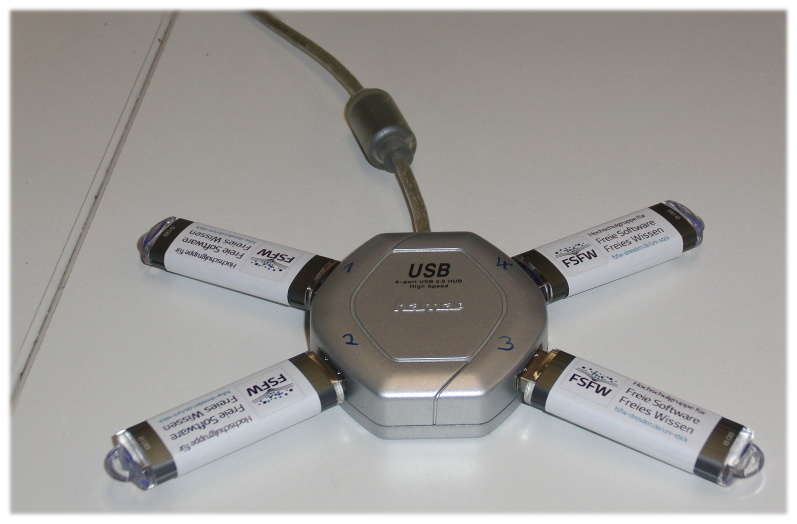
\includegraphics[width=40mm]{img-src/usb-hub}
    }
  \end{textblock*}

  \begin{textblock*}{55mm}[0.,0.](15mm,50mm)
    \visible<3->{
      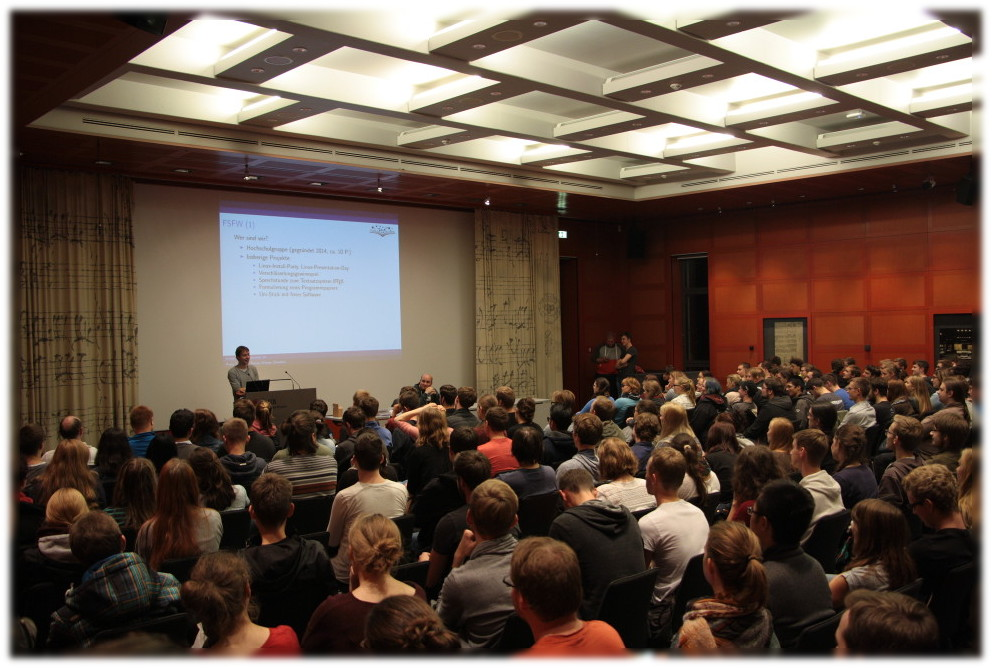
\includegraphics[width=55mm]{img-src/uni-stick-ausgabe-vortrag}
    }
  \end{textblock*}

  \begin{textblock*}{55mm}[0.,0.](71mm,63mm)
    \visible<4->{
      \begin{itemize}
       \item Accessibility:
       \hspace{-5mm}
       \begin{itemize}
        \item brltty
        \item gnome-orca (Screenreader)
        \item ...
        \item WIP!
       \end{itemize}



      \end{itemize}

    }
  \end{textblock*}

\end{frame}

%%%%%%%%%%%%%%%%%%%%%%%%%%%%%%%%%%%%%%%%%%%%%%%%%%%%%%%%%%%%%%%%%%%%%%%%%%%%%%%%

\begin{frame}[label=ct3]
  \frametitle{Zukunftsideen}

  \begin{itemize}
  \item Fortführung "`Uni-Stick"'
  \item Studierende zum Nutzen/Verbessern freier Software animieren
    \begin{itemize}
    \item Mehr Blog-Beiträge
    \item Kurse (\LaTeX / Python /\textbf{ Git} / Inkscape / \dots)
    \item Ansible-Infrastruktur-Stipendium
    \item OpenSource-Wettbewerb/Preis
    \item \dots
    \end{itemize}

    \bigskip

  \item Aufmerksamkeit erzeugen / Lobby-Arbeit

    \bigskip

  \item Vernetzung mit anderen Städten

  \end{itemize}

\end{frame}

%%%%%%%%%%%%%%%%%%%%%%%%%%%%%%%%%%%%%%%%%%%%%%%%%%%%%%%%%%%%%%%%%%%%%%%%%%%%%%%%

\begin{frame}[label=ct4]
  \frametitle{Weitere Informationen}

  \onslide<+->

  \begin{center}
    \url{https://fsfw-dresden.de/}
    % HACK THE PLANET!
    $\;\;\left\{\;\;\text{
        \parbox{2.3cm}{
          \texttt{uni-stick}\\[1mm]
          \texttt{blog}\\[1mm]
          \texttt{newsletter}
          \texttt{mitmachen}\\[1mm]
          \texttt{fork}\\[-3mm]
        }}
    \right.$

    \vspace*{2\bigskipamount}

    
\includegraphics[width=50mm]{img-src/fsfw-netzwerke}
  \end{center}

\end{frame}

%%%%%%%%%%%%%%%%%%%%%%%%%%%%%%%%%%%%%%%%%%%%%%%%%%%%%%%%%%%%%%%%%%%%%%%%%%%%%%%%
\begin{frame}[label=wb2]

\begin{center}
 \vspace{10mm}
\structure{\Huge  </Eigenwerbung>}
\end{center}

\end{frame}

%%%%%%%%%%%%%%%%%%%%%%%%%%%%%%%%%%%%%%%%%%%%%%%%%%%%%%%%%%%%%%%%%%%%%%%%%%%%%%%%

\begin{frame}[label=ol1]
  \frametitle{Gliederung}
  \tableofcontents
\end{frame}

%%%%%%%%%%%%%%%%%%%%%%%%%%%%%%%%%%%%%%%%%%%%%%%%%%%%%%%%%%%%%%%%%%%%%%%%%%%%%%%%
\section{Warum Versionsverwaltung?}

\begin{frame}[label=why10]
\frametitle{Warum Versionsverwaltung?}

\begin{itemize}
  \item Projekte bestehen aus schrittweisen Änderungen
  \item Bedürfnis, zu vorherigem Zustand zurückkehren zu können

  \begin{itemize}
\item  ("`Savegame"')
    \end{itemize}

  \item Naiver Ansatz: \hspace{10mm}
  \raisebox{-0.5\height}{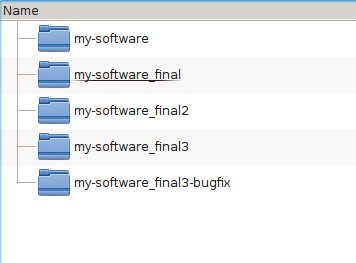
\includegraphics[width=40mm]{img-src/my-software-dirs}}

  \item Probleme:
  \begin{itemize}
   \item Speicherplatz
   \item Fehlende Übersicht
   \item Skaliert nicht (Teamwork)
  \end{itemize}

  \end{itemize}
\end{frame}

%%%%%%%%%%%%%%%%%%%%%%%%%%%%%%%%%%%%%%%%%%%%%%%%%%%%%%%%%%%%%%%%%%%%%%%%%%%%%%%%
% TODO: image source http://techidiocy.com/understand-git-clone-command-svn-checkout-vs-git-clone/
% https://softwareengineering.stackexchange.com/questions/136079/are-there-any-statistics-that-show-the-popularity-of-git-versus-svn
% http://www.wastedpotential.com/version-control-throwdown-git-vs-svn/
\section{Warum Git?}
\begin{frame}[label=why20]
\frametitle{Warum Git? (1)}

\begin{itemize}
  \item Lösung 1: zentrale Versionsverwaltung
  \begin{itemize}
   \item CVS (1986), SVN (2000)
   \item Idee: Zentrales Repositorium und Arbeitskopien \\[1ex]
       \hspace*{1cm}\begin{tikzpicture}[%
           node distance=2cm and 1cm,
           location/.style={
             % The shape:
             rectangle,
             % The size:
             minimum size=6mm,
             % The border:
             very thick,
             draw=red!50!black!50,
             % 50% red and 50% black,
             % and that mixed with 50% white
             % The filling:
             top color=white,
             % a shading that is white at the top...
             bottom color=red!50!black!20, % and something else at the bottom
           },
           checkout/.style={
             <->,
             shorten <=2pt,
             shorten >=2pt,
             thick,
             color=black!40!white,
           }]

         ]
         \node[location, draw=green!50!black!50, bottom color=green!50!black!20] (repository) {SVN Repo};
         \node[location] (user1) [below left of=repository] {Arbeitskopie 1};
         \node[location] (user2) [below of=repository, yshift=-1ex] {Arbeitskopie 2};
         \node[location] (user3) [below right of=repository] {Arbeitskopie 3};

         \draw[checkout] ($ (repository.south) + (-2pt, 0) $) -- (user1.north);
         \draw[checkout] (repository.south) -- (user2.north);
         \draw[checkout] ($ (repository.south) + (2pt, 0) $) -- (user3.north);
       \end{tikzpicture}
   \end{itemize}
  \item Probleme:
  \begin{itemize}
   \item Abhängig von Server-Erreichbarkeit
   \item Performanz
  \end{itemize}

  \end{itemize}
\end{frame}

%%%%%%%%%%%%%%%%%%%%%%%%%%%%%%%%%%%%%%%%%%%%%%%%%%%%%%%%%%%%%%%%%%%%%%%%%%%%%%%%
\begin{frame}[label=why30]
\frametitle{Warum Git? (2)}

\begin{itemize}
  \item Lösung 2: \textbf{de}zentrale Versionsverwaltung
  \begin{itemize}
   \item mercurial (2005), bazaar (2005) \textbf{git} (2005)
   \item Idee: Jeder hat ein vollwertiges Repositorium \\[1ex]
      \hspace*{1cm}\begin{tikzpicture}[%
           node distance=2cm and 1cm,
           location/.style={
             % The shape:
             rectangle,
             % The size:
             minimum size=6mm,
             % The border:
             very thick,
             draw=green!50!black!50,
             % 50% red and 50% black,
             % and that mixed with 50% white
             % The filling:
             top color=white,
             % a shading that is white at the top...
             bottom color=green!50!black!20, % and something else at the bottom
           },
           checkout/.style={
             <->,
             shorten <=2pt,
             shorten >=2pt,
             thick,
             color=black!40!white,
           }]

         ]
         \node[location] (user1) {Git Repo 1};
         \node[location] (user2) [below  left of=user1] {Git Repo 2};
         \node[location] (user3) [below right of=user1] {Git Repo 3};

         \draw[checkout] ($ (user1.south) + (-2pt, 0) $) -- (user2.north);
         \draw[checkout] (user3.west) -- (user2.east);
         \draw[checkout] ($ (user1.south) + (2pt, 0) $) -- (user3.north);

     \end{tikzpicture}
  \end{itemize}
  \item Vorteile:
  \begin{itemize}
   \item Alle Operationen lokal $\rightarrow$ schnell, unabhängig
   \item Einfaches "`branching"' und "`merging"'
   \item ...
  \end{itemize}
  \end{itemize}
\end{frame}

%%%%%%%%%%%%%%%%%%%%%%%%%%%%%%%%%%%%%%%%%%%%%%%%%%%%%%%%%%%%%%%%%%%%%%%%%%%%%%%%
\begin{frame}[label=why40]
\frametitle{Warum Git? (3)}

\begin{textblock*}{\textwidth}[0.5,0.](60mm,20mm)
\begin{center}%
\only<1>{
\begin{figure}
  
\includegraphics[width=80mm]{img-src/svn-vs-git-boxing}
\end{figure}
}
\only<2->{
\begin{figure}
  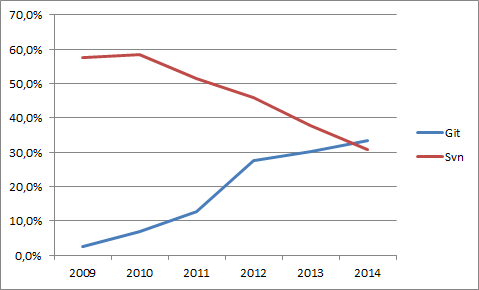
\includegraphics[width=80mm]{img-src/svn-vs-git-stats}\\
%   \caption{Git and SVN \$WHATISPLOTTEDHERE} %% "Abbildung:" Unnötig
{Gefühlter Grad der Verbreitung: Git vs SVN}
\end{figure}
}
\bigskip
\visible<3->
{
2017: Git = defacto Standard
}
\end{center}
\end{textblock*}


\end{frame}

%%%%%%%%%%%%%%%%%%%%%%%%%%%%%%%%%%%%%%%%%%%%%%%%%%%%%%%%%%%%%%%%%%%%%%%%%%%%%%%%
\section{Git Einführung (mit Praxis)}
\begin{frame}
\frametitle{Einführung in git – Was ist ein Repo?}
\begin{columns}
  \column{0.245\textwidth}
  \begin{tikzpicture}
    \gitDAG[grow down sep = 1em]{
      A -- B -- C
    };
    \gitbranch{master}{left=of C}{C};
    \gitHEAD{above=of master}{master}
    \SAandWT
  \end{tikzpicture}
  \column{0.75\textwidth}
  \begin{itemize}
  \item gerichteter, azyklischer Graph von Versionen
    (\emph{revisions}) einer Ordnerstruktur und deren Inhalt mit
    Metadaten (\emph{Commit-ID}, Autor, Beschreibungstext)
  \item Commit-ID abgeleitet aus dem Inhalt und dem Graphen
    (kryptographische Hash-Funktion)
  \item \emph{\texttt{HEAD}}: Knoten im Graphen; momentaner
    Bezugspunkt für Operationen
  \item \emph{refs}: referenzieren Knoten im Graphen (Beispiele:
    \texttt{HEAD}, \texttt{HEAD\^}, \texttt{master}, per abgekürzter
    Commit-ID \texttt{f23faaa})
  \end{itemize}
\end{columns}
\end{frame}

\begin{frame}[label=gitintro10]
\frametitle{Einführung in git – Verwendung}
\begin{itemize}
 \item Wir empfehlen: git Bedienung via Kommandozeile
   %% NOTES:
   % \begin{itemize}
   % \item Alternative: Integration in die IDE
   % \item Kommandozeile kann mehr
   % \item[$\Rightarrow$] können hilft oft weiter
   % \end{itemize}
 \item Syntax: \texttt{git <command> [<args>]}
 \item Beispiele:

 \begin{itemize}
  \item \texttt{git init}
  \item \texttt{git add myscript.py}
  \item \texttt{git commit -m "{}add basic functionality"}
  \item \texttt{git push}\\[2mm]
  \pause
  \item \texttt{git status}
  \item \texttt{git log}
  \item \texttt{git branch develop}
  \item \texttt{git checkout master}
  \item \texttt{git merge develop}
  \item \texttt{git blame myscript.py}
  \item \texttt{git diff}
  \item \texttt{git difftool}

 \end{itemize}
\end{itemize}

\begin{textblock*}{\textwidth}[0.5,0.](120mm, 60mm)

\visible<3->{
\begin{itemize}
 \item[] ~
\begin{itemize}

  \item \texttt{git clone}
  \item \texttt{git help <command>}
  \item \texttt{git rebase} \\[2mm]
  \item \texttt{git config}

  \item \texttt{gitk}

\end{itemize}
\end{itemize}
}
\end{textblock*}

\end{frame}

%%%%%%%%%%%%%%%%%%%%%%%%%%%%%%%%%%%%%%%%%%%%%%%%%%%%%%%%%%%%%%%%%%%%%%%%%%%%%%%%

\begin{frame}[label=gitintro20]
\frametitle{Praxis 1: Erste Schritte}
\begin{itemize}
 \item Konfiguration anpassen
 \begin{itemize}
  \item \texttt{git config -{}-global user.email "foo@bar.de"}
  \item \texttt{git config -{}-global user.name "Your Name"}
  \item ...
 \end{itemize}

 \item Eigenes Repo \texttt{foo} erstellen
 \begin{itemize}
  \item \texttt{mkdir foo}
  \item \texttt{cd foo}
  \item \texttt{git init}
 \end{itemize}
 \item Alternativ: Bestehenedes Repo klonen
 \begin{itemize}
  \item \texttt{git clone <url>}
 \end{itemize}
 \item[]
 \pause
 \item Hintergrund: Wo speichert git die relevanten Informationen?
 \item[$\rightarrow$] Verstecktes Verzeichnis:
 \raisebox{-0.5\height}{
 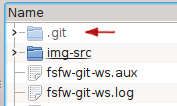
\includegraphics[width=20mm]{img-src/git-dir1}}


\end{itemize}

\end{frame}
%%%%%%%%%%%%%%%%%%%%%%%%%%%%%%%%%%%%%%%%%%%%%%%%%%%%%%%%%%%%%%%%%%%%%%%%%%%%%%%%

\begin{frame}
  \frametitle{Theorie: typischer Ablauf / "`staging area"' (1)}
  \begin{center}
    %% Gehirnvirus zuerst und allein auf einer Folie
    %% Details mit schema auf einer späteren folie
    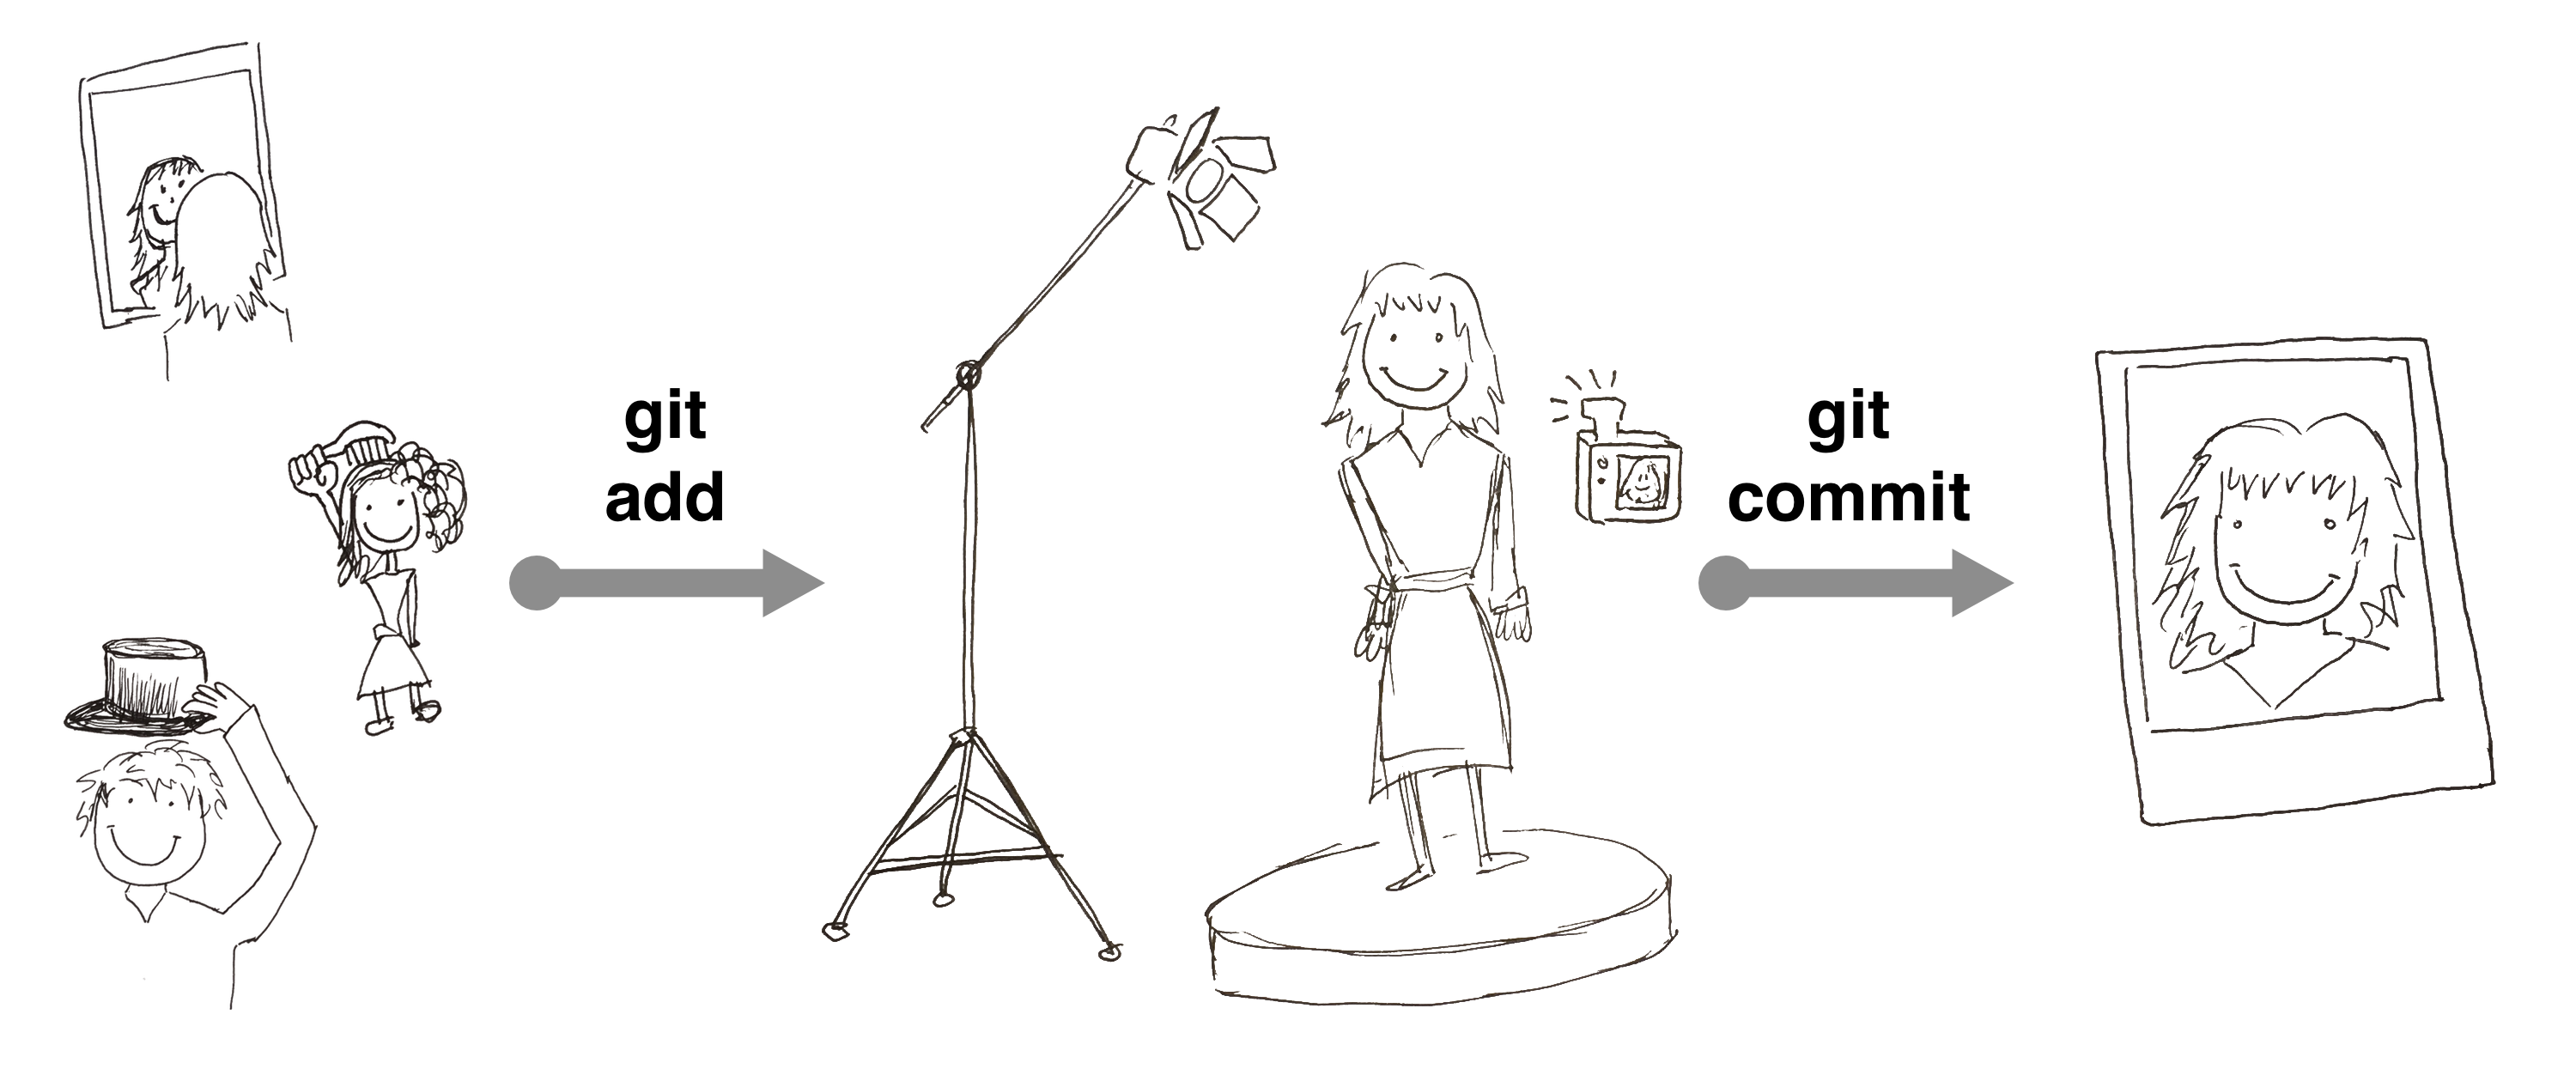
\includegraphics[width=80mm]{img-src/git-staging-area}
  \end{center}
\end{frame}

\begin{frame}[label=gitintro30]
\frametitle{Theorie: typischer Ablauf / "`staging area"' (2)}
\vspace{-8mm}
\begin{center}
  \begin{tikzpicture}[
    every text node part/.style={align=center},
    node distance=3cm,
    location/.style={
      % The shape:
      rectangle,
      % The size:
      minimum size=6mm,
      % The border:
      very thick,
      draw=red!50!black!50,
      % 50% red and 50% black,
      % and that mixed with 50% white
      % The filling:
      top color=white,
      % a shading that is white at the top...
      bottom color=red!50!black!20, % and something else at the bottom
      text height=4ex,
      text depth=0.25ex,
    }]

    \node[location] (untracked) {working \\ tree};
    \node[location] (staged) [right of=untracked] {index \\[-0.7em]};
    \node[location] (committed) [right of=staged] {local \\ repository};
    \node[location] (published) [right of=committed] {remote \\ repository};

    \draw[->, thick, color=black!40!white] (untracked.east) -- (staged.west)
          node [midway, above=2.5ex, color=black] {\texttt{git add}};
    \draw[->, thick, color=black!40!white] (staged.east) -- (committed.west)
          node [midway, above=2.5ex, color=black] {\texttt{git commit}};
    \draw[->, thick, color=black!40!white] (committed.east) -- (published.west)
          node [midway, above=2.5ex, color=black] {\texttt{git push}};
  \end{tikzpicture}
\end{center}
Wozu zweiphasiger Commit-Prozess?
\begin{itemize}
 \item Ermöglicht präzise, hoch aufgelöste Commits\\
 \begin{itemize}
  \item Änderungen mancher Dateien (\texttt{git add dir1/*.html})
  \item Nur bestimmte Änderungen einer Datei (\texttt{git add -p})
  \item Alle Änderungen übernehmen und comitten (\texttt{git commit -a})
 \end{itemize}
 \item[$\Rightarrow$] nachvollziehbare, aussagekräftige Commit-History
\end{itemize}


\end{frame}

%%%%%%%%%%%%%%%%%%%%%%%%%%%%%%%%%%%%%%%%%%%%%%%%%%%%%%%%%%%%%%%%%%%%%%%%%%%%%%%%
\begin{frame}[fragile,label=gitintro40]
\frametitle{Praxis: minimales Repo}
\vspace{-5mm}
\begin{columns}
% Trick: durch Einfügen einer weiteren Spalte wird die 1. Spalte nach links gedrückt
\column[t]{1.0\textwidth}
\begin{itemize}
 \item Inhalt erzeugen
\begin{itemize}
 \item \verb|printf "Hallo\nWelt\n" > README.md|
 \item \texttt{git status}
 \item \texttt{git add README.md} \qquad \visible<1->{{\scriptsize Tipp: Auto-Vervollständigung mit TAB}}
 \item \texttt{git status}
 \item \verb|git commit -m "New content of README"| %\quad \visible<4->{{\scriptsize Fehler absichtlich}}
 \item \texttt{git status}
\end{itemize}
\pause
 \item Änderungen durchführen, anzeigen und committen
\begin{itemize}
 \item \verb|sed -i -- "s/Welt/Leute/g" README.md|
 \item \texttt{git diff}
 \pause
 \pause
 \item \texttt{git commit --add -m "{}change Hello-message"{}}
\end{itemize}
 \pause
 \item Sich Überblick verschaffen
 \begin{itemize}
 \item \texttt{git status}
 \item \texttt{git log}
 \item \texttt{gitk}
 \end{itemize}
%  \pause
%  \item Letzten commit korrigieren (mit Editor, default: \texttt{\$EDITOR})
%  \begin{itemize}
%  \item  \texttt{git config -{}-global core.editor mcedit}
%  \item \texttt{git commit -{}-amend}
%  \end{itemize}
\end{itemize}

\column[t]{0.1\textwidth}
~
\end{columns}


\begin{textblock*}{1cm}[0.,0.](95mm,53mm)
\visible<3->{
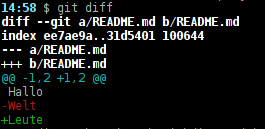
\includegraphics[height=15mm]{img-src/git-diff-snapshot}
}
\end{textblock*}

\end{frame}

%%%%%%%%%%%%%%%%%%%%%%%%%%%%%%%%%%%%%%%%%%%%%%%%%%%%%%%%%%%%%%%%%%%%%%%%%%%%%%%%
\begin{frame}[label=branches10]
\frametitle{Theorie: Branches}
\begin{columns}
\column{0.349\textwidth}
\only<1,2>{
\begin{tikzpicture}
      \useasboundingbox (-1.5,-4.5) rectangle +(4,4.5);

      % Commit DAG
      \gitDAG[grow down sep = 1em]{
        A -- B -- C
      };
      % Branch

      \gitbranch
        {master}     % node name and text
        {left=of C} % node placement
        {C}          % target
      % HEAD reference
      \gitHEAD
        {above=of master} % node placement
        {master}          % target
    \end{tikzpicture}
}
\only<3,5>{
\begin{tikzpicture}
     \useasboundingbox (-1.5,-4.5) rectangle +(4,4.5);

      % Commit DAG
      \gitDAG[grow down sep = 1em]{
        A -- B --{
              C,
              D -- E,
        }
      };
      % Branch

      \gitbranch
        {master}     % node name and text
        {left=of C} % node placement
        {C}          % target
      % HEAD reference
      \gitHEAD
        {above=of master} % node placement
        {master}          % target

      \gitbranch
        {bugfix}     % node name and text
        {left=of E} % node placement
        {E}
    \end{tikzpicture}
} % end of only
\only<4,6>{
\begin{tikzpicture}
      \useasboundingbox (-1.5,-4.5) rectangle +(4,4.5);

      % Commit DAG
      \gitDAG[grow down sep = 1em]{
        A -- B --{
              C,
              D -- E,
        }
      };

      % Branch
      \gitbranch
        {master}     % node name and text
        {left=of C} % node placement
        {C}          % target
      % HEAD reference
      \gitHEAD
        {below=of bugfix} % node placement
        {bugfix}          % target

      \gitbranch
        {bugfix}     % node name and text
        {left=of E} % node placement
        {E}
    \end{tikzpicture}
} % end of only
\only<7>{
\begin{tikzpicture}
      \useasboundingbox (-1.5,-4.5) rectangle +(4,4.5);

      % Commit DAG
      \gitDAG[grow down sep = 1em]{
        A -- B --{
              C,
              D -- E,
        }
      };

      % Branch
      \gitbranch
        {master}     % node name and text
        {left=of C} % node placement
        {C}          % target
      \gitbranch
        {bugfix}     % node name and text
        {left=of E} % node placement
        {E}

      \gitHEAD
        {above=of D, xshift=1.5em} % node placement
        {D}
    \end{tikzpicture}
} % end of only
\only<8>{
\begin{tikzpicture}
      \useasboundingbox (-1.5,-4.5) rectangle +(4,4.5);

      % Commit DAG
      \gitDAG[grow down sep = 1em]{
        A -- B --{
              C,
              D -- E,
        }
      };

      % Branch
      \gitbranch
        {master}     % node name and text
        {left=of C} % node placement
        {C}          % target
      \gitbranch
        {bugfix}     % node name and text
        {left=of E} % node placement
        {E}

      \gitbranch
        {experiment}     % node name and text
        {above=of D, xshift=1.5em} % node placement
        {D}
      % HEAD reference
      \gitHEAD
        {above=of experiment} % node placement
        {experiment}          % target

    \end{tikzpicture}
} % end of only
\only<9>{
\begin{tikzpicture}
      \useasboundingbox (-1.5,-4.5) rectangle +(4,4.5);

      % Commit DAG
      \gitDAG[grow down sep = 1em]{
        A -- B --{
              C,
              D --{ E,
                    F -- G,
                  }
        }
      };


      % Branch
      \gitbranch
        {master}     % node name and text
        {left=of C} % node placement
        {C}          % target
      \gitbranch
        {bugfix}     % node name and text
        {left=of E} % node placement
        {E}

      \gitbranch
        {experiment}     % node name and text
        {left=of G} % node placement
        {G}
      % HEAD reference
      \gitHEAD
        {left=of experiment} % node placement
        {experiment}          % target

    \end{tikzpicture}
} % end of only
\column{0.65\textwidth}
\begin{itemize}
\item Unkompliziertes paralleles Arbeiten an verschieden Versionen
\item<2-> Der aktive Branch folgt \texttt{HEAD}
\item<3-> beliebig viele Branches möglich
\item<4-> Branch/Revision wechseln:\\ \texttt{git checkout \only<4,6>{bugfix}\only<5>{master}\only<7,8,9>{<ref>}}
\item<8-> neuer Branch auf \texttt{HEAD} erstellen:\\ \texttt{git checkout -b experiment}
\end{itemize}
\end{columns}
\end{frame}

\begin{frame}
\frametitle{Theorie: Zusammenfassung Branches}
\begin{columns}
  \column{0.349\textwidth}
\begin{tikzpicture}
      \useasboundingbox (-1.5,-4.5) rectangle +(4,4.5);

      % Commit DAG
      \gitDAG[grow down sep = 1em]{
        A -- B --{
              C,
              D --{ E,
                    F -- G,
                  }
        }
      };

      % Branch
      \gitbranch
        {master}     % node name and text
        {left=of C} % node placement
        {C}          % target
      \gitbranch
        {bugfix}     % node name and text
        {left=of E} % node placement
        {E}

      \gitbranch
        {experiment}     % node name and text
        {left=of G} % node placement
        {G}
      % HEAD reference
      \gitHEAD
        {left=of experiment} % node placement
        {experiment}          % target

    \end{tikzpicture}

  \column{0.65\textwidth}
  \begin{center}
    \Large Branches sind \emph{lokale} Lesezeichen auf Knoten im
    Revisionsgraphen. Beim Anlegen eines neuen Commits folgt der aktive
    Branch dem neuen \texttt{HEAD}.
  \end{center}
\end{columns}
\end{frame}

%%%%%%%%%%%%%%%%%%%%%%%%%%%%%%%%%%%%%%%%%%%%%%%%%%%%%%%%%%%%%%%%%%%%%%%%%%%%%%%%

% noch nich fertig/sinnvoll
% \begin{frame}[label=komplex10]
% \frametitle{Beispiel-Repo: lyrik}
% \begin{itemize}
%  \item Bereitgestelltes nicht-trivials Repo URL:
%  \item Basis für verschiedene Aufgaben
% \begin{enumerate}
%  \item Repo konen \texttt{git clone <url>}
%  \item Überblick verschaffen
%  \begin{enumerate}
%   \item Wie viele Commits, Committer
%   Branches?
%
%  \end{enumerate}
%
% \end{enumerate}
%
% \end{itemize}
%
% \end{frame}


% # Notizen zur Aufgabenstellung:
%
% repo klonen
% Überblick verschaffen (gitk --all)
% zum Branch weimar wechseln und 'YYY' durch 'ich' ersetzen
% zum Branch london wechseln und 'XXX' durch 'thee' ersetzen, commiten
% mit git blame herausfinden, wann welche Zeile von wem zuletzt editiert wurde
%  git blame AUTHORS.md
%  git blame sonnets/text1.md
%
% Änderrungen seit dem vorletzten commit anzeigen: git diff HEAD~
% Manuelle Änderungen vornehmen
% Änderungen seit dem letzten commit anzeigen
%
% Optional: git difftool dazu verwenden
%
% Branch london in branch master mergen
% Branch weimar in branch master mergen
%
% ausführen: python3 scripts/find-shortest-poem
% git status -> Problem mit __pycache__
% passende .gitignore Datei anlegen
%
% Branch rom in branch master mergen -> Manuellen Konflikt beheben.
%
%
% Für Fortgeschrittene: das ganze repo mittels git rebase zu einem unverzwiegten umwandeln
%

%%%%%%%%%%%%%%%%%%%%%%%%%%%%%%%%%%%%%%%%%%%%%%%%%%%%%%%%%%%%%%%%%%%%%%%%%%%%%%%%

\begin{frame}[label=gitintro50]
\frametitle{Noch fehlende Inhalte (kurz oder mit eigener Folie)}
\begin{itemize}
\item diff \checkmark / difftool
\item branches \checkmark
\item Visualisierung eines repos (Graph mit Pfeilen) \checkmark
\item HEAD\checkmark , hash bzw. ref
\item merge (Konflikte),  erwähnen: push, fast-forward, rebase,
\item .gitignore
\item github $\neq$ git
\item git nicht gut für Binärdateien
\item bash extension
\item aliase in .gitconfig
\item link auf branching model
\item globale gitignore

\end{itemize}
\end{frame}

%%%%%%%%%%%%%%%%%%%%%%%%%%%%%%%%%%%%%%%%%%%%%%%%%%%%%%%%%%%%%%%%%%%%%%%%%%%%%%%%

\begin{frame}[label=link10]{Tipps und Links}
Weitere Ressourcen:
\tiny
\begin{itemize}
 \item
\url{https://learn.adafruit.com/an-introduction-to-collaborating-with-version-control/initializing-a-repository-and-making-commits}
\item ...
\end{itemize}


\end{frame}




%%%%%%%%%%%%%%%%%%%%%%%%%%%%%%%%%%%%%%%%%%%%%%%%%%%%%%%%%%%%%%%%%%%%%%%%%%%%%%%%
\begin{frame}[label=uj]{Ausblick}
\begin{itemize}
 \item Fragen?\\[10mm]
   \pause
 \item Unterstützung später {\tiny (im Rahmen unserer Möglichkeiten)}:
   \begin{itemize}
   \item \url{https://fsfw-dresden.de/sprechstunde}
   \item \url{kontakt@fsfw-dresden.de}
   \end{itemize}
\end{itemize}



\end{frame}

%%%%%%%%%%%%%%%%%%%%%%%%%%%%%%%%%%%%%%%%%%%%%%%%%%%%%%%%%%%%%%%%%%%%%%%%%%%%%%%%
\end{document}
